\newtheorem{definisi}{Definisi}
\newtheorem{proposisi}{Proposisi}
\newtheorem{aksioma}{Aksioma}
\chapter{Teori Permainan}
\section{Teori Permainan}
%bahas game theory
Menurut \textcite{tadelis2013game}, teori permainan merupakan ilmu yang mempelajari pemodelan matematis untuk masalah dan kerja sama antara agen pengambil keputusan. Pengambil keputusan yang selanjutnya disebut sebagai pemain umumnya memiliki informasi yang berguna untuk proses pengambilan keputusan selanjutnya. Pemain harus mengetahui tiga hal yang mendasari masalah ini, seperti: Apa saja pilihan yang mungkin dilakukan? Apa saja hasil dari setiap pilihan? Bagaimana dampak dari hasil tersebut?

Pengamatan sederhana diatas memberikan definisi pertama yang penting untuk setiap masalah pengambilan keputusan.
\begin{definisi}
    \textbf{Masalah pengambilan keputusan} terdiri atas tiga komponen penting:
    \begin{enumerate}
        \item \textbf{Aksi}, yaitu seluruh alternatif pilihan yang dapat dilakukan pemain.
        \item \textbf{Payoff} atau \textbf{bayaran}, yaitu seluruh konsekuensi yang dapat terjadi dari aksi.
        \item \textbf{Preferensi}, yaitu deskripsi bagaimana pemain mengurutkan himpunan keluaran dari yang paling diinginkan hingga paling tidak diinginkan.
    \end{enumerate}
\end{definisi}

\begin{proposisi}
    Jika himpunan keluaran X berhingga, maka suatu relasi preferensi rasional X dapat direpresentasikan sebagai fungsi payoff.
\end{proposisi}

Berikut ini diagram alir yang menyatakan bagaimana pengambilan keputusan diambil.
\pagebreak
\begin{figure}
    \centering
    \tikzstyle{terminal} = [rectangle, rounded corners, draw=black, fill=blue!30, inner sep=.2cm, text width=3.5cm, align=flush center]
\tikzstyle{others} = [rectangle, text centered, draw=black, inner sep=.2cm, align=flush center, text width=2.5cm]
\tikzstyle{arrow} = [draw, thick, ->, >=stealth]

\newcommand{\factorcolor}{red!30}
\newcommand{\externalcolor}{cyan!10}
\newcommand{\payoffcolor}{green!20}

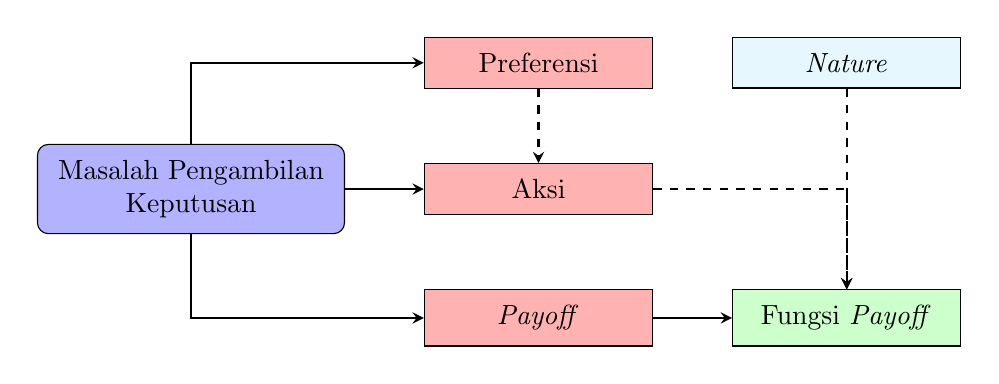
\begin{tikzpicture}[node distance=2cm]
  \matrix[column sep=1cm, row sep=7mm]{
                                                           & \node (pref) [others, fill=\factorcolor] {Preferensi};           &
    \node (nat) [others, fill=\externalcolor] {\textit{Nature}};                                                          \\
    \node (dp) [terminal] {Masalah Pengambilan Keputusan}; &
    \node (act) [others, fill=\factorcolor] {Aksi};        &                                                                    \\
                                                           & \node (po) [others, fill=\factorcolor] {\textit{Payoff}}; &
    \node (fpo) [others, fill=\payoffcolor] {Fungsi \textit{Payoff}};                                                    \\
  };

  \begin{scope}[every path/.style=arrow]
    \path (dp) -- (act);
    \path (dp) |- (pref);
    \path (dp) |- (po);
    \path (po) -- (fpo);
    \path [dashed] (pref) -- (act);
    \path [dashed] (act) -| (fpo);
    \path [dashed] (nat) -- (fpo);
  \end{scope}
\end{tikzpicture}
    \caption{Diagram Alir Masalah Pengambilan Keputusan}
\end{figure}

Relasi preferensi dinyatakan dalam notasi $\succsim$, yang menyatakan relasi antar \textit{payoff} yang dapat menunjukkan preferensi pemain. Sebagai contoh, misalkan terdapat seorang pemain yang ingin memilih rasa es krim vanila atau stroberi. Pilihan rasa es krim ini dapat di lambangkan sebagai himpunan aksi yang akan dipilih pemain yaitu  $A = \lbrace v, s\rbrace$, di mana $v$ menyatakan rasa vanila dan $s$ menyatakan rasa stroberi. Aksi yang dipilih pemain dapat berupa kondisi di mana pemain memutuskan untuk memakan es krim rasa vanila atau stroberi. Hal ini dapat ditulis sebagai himpunan bayaran $P = \lbrace V, S\rbrace$.

\begin{aksioma}
    \textbf{Relasi preferensi} $\succsim$ dikatakan \textbf{lengkap} jika untuk setiap keluaran $x,\space y \in X$ bisa diurutkan berdasarkan relasi preferensi, yaitu $x \succsim y$ atau $y \succsim x$.
\end{aksioma}

Asumsikan bahwa pemain ini lebih memilih rasa es krim yang ia sukai yaitu es krim rasa vanila, namun tidak mempermasalahkan kondisi ketika ia mendapatkan rasa stroberi. Maka dapat digunakan notasi $V \succsim S$, yang bermakna "pemain menyukai es krim rasa vanila lebih dari atau sama dengan rasa stroberi". Notasi $S \succsim V$ digunakan apabila pemain tersebut memiliki preferensi sebaliknya.
Apabila keluaran tersebut dapat ditulis sebagai $V \succsim S$ atau $S \succsim V$, relasi preferensi dikatakan bersifat lengkap.

Jika pemain ini menyatakan bahwa ia lebih menyukai es krim rasa vanila dibandingkan rasa stroberi dan pasti akan memilih es krim rasa vanila apabila dihadapi pilihan dua rasa tersebut, pernyataan ini dinotasikan dengan $V \succ S$. Jika pemain ini tidak dapat memilih rasa yang disukai karena tingkat kesukaan sama, artinya relasi preferensi ditulis sebagai $V \sim S$.

\begin{aksioma}
    \textbf{Relasi preferensi} $\succsim$ dikatakan \textbf{transitif} jika untuk setiap keluaran $x,\space y, \space z \in X$, jika $x \succsim y$ dan $y \succsim z$, maka $x \succsim z$.
\end{aksioma}

Untuk masalah yang serupa, misalkan pemain yang sama harus memilih rasa es krim vanila, stroberi, atau durian. Pemain tersebut tidak mempermasalahkan kondisi ketika ia mendapatkan rasa es krim apapun.
Namun berdasarkan tingkat kesukaan, pemain tersebut memilih rasa vanila, durian, kemudian stroberi. Misalkan $A = \lbrace v, d, s\rbrace$ adalah himpunan aksi yang dipilih pemain  dan $P = \lbrace V, D, S\rbrace$ adalah himpunan bayaran. Maka relasi preferensi untuk kondisi diatas dapat ditulis sebagai $V \succsim D$ dan $D \succsim S$, sehingga $V \succsim S$. Artinya, relasi preferensi untuk masalah ini dikatakan bersifat transitif.

Dalam masalah pengambilan keputusan terdapat sifat tidak pasti yang sulit atau tidak dapat distrategikan oleh pemain. Sifat tidak pasti ini disebut sebagai \textbf{sifat alamiah} atau \textbf{\textit{nature}}. Pemain harus dapat membuat strategi dengan mempertimbangkan \textit{nature} permainan.

\section{Teori Permainan Berdasarkan Kelengkapan Infomasi}
Dalam memainkan suatu permainan, informasi menjadi hal yang penting untuk diketahui pemain. Informasi permainan membantu pemain untuk mendapatkan gambaran permainan, batasan permainan, serta aturan-aturan yang harus diikuti dalam permainan tersebut. Dengan memahami informasi permainan dengan baik, pemain dapat mengoptimalkan strategi permainan dan meminimalisir terjadinya kesalahan yang dapat merugikan pemain. Namun, informasi dalam permainan terkadang tidak sepenuhnya diberikan. Misalnya,informasi yang diberikan permainan bukanlah \textbf{pengetahuan umum}.

\begin{definisi}
    Sebuah kejadian merupakan \textbf{pengetahuan umum} jika:
    \begin{enumerate}
        \item Kejadian diketahui seluruh pemain.
        \item Seluruh pemain tahu bahwa kejadian tersebut diketahui seluruh pemain.
              %\item \textit{ad infinitum}.
    \end{enumerate}
\end{definisi}

Berdasarkan kelengkapan informasi, teori permainan dibagi menjadi teori permainan dengan informasi lengkap dan teori permainan dengan informasi tidak lengkap.

%Permainan dengan Informasi Lengkap
\subsection{Permainan dengan Informasi Lengkap}
Salah satu permainan dengan informasi lengkap adalah catur. Permainan catur adalah permainan papan yang dimainkan oleh dua pemain dengan menggerakan 16 bidak secara bergantian di papan persegi. Tujuan dari permainan catur adalah menyerang raja lawan sehingga raja lawan tidak bisa bergerak, atau berada di posisi "skak-mat". Dalam permainan catur, 16 bidak yang dimiliki pemain pertama dan pemain kedua sama. Artinya, setiap pemain mengetahui seluruh kemungkinan aksi dan seluruh kemungkinan keluaran yang dilakukan pemain lainnya. Akibatnya, setiap pemain juga mengetahui dapat mengetahui \textit{payoff} serta kemungkinan preferensi pemain lain dari aksi yang dilakukan. Oleh karena itu, permainan catur disebut sebagai permainan dengan informasi lengkap. Permainan dengan informasi lengkap didefinisikan sebagai berikut.
\begin{definisi}
    \textbf{Permainan dengan informasi lengkap} adalah permainan di mana komponen berikut merupakan \textbf{pengetahuan umum} bagi seluruh pemain:
    \begin{enumerate}
        \item Seluruh kemungkinan aksi yang dilakukan seluruh pemain.
        \item Seluruh kemungkinan keluaran.
        \item Bagaimana setiap kombinasi aksi pemain mempengaruhi keluaran.
        \item Preferensi setiap dan seluruh pemain terhadap keluaran.
    \end{enumerate}
\end{definisi}

Selain catur, beberapa contoh permainan dengan informasi lengkap adalah \textit{Prisoner's Dilemma}, \textit{Game of Chicken}, dan \textit{Tic-Tac-Toe}. Permainan \textbf{Persona 4 Golden} juga merupakan permainan dengan informasi lengkap.

%Permainan dengan Informasi Tidak Lengkap
\subsection{Permainan dengan Informasi Tidak Lengkap}
Ketika bermain beberapa jenis permainan, seringkali pemain tidak mengetahui atau tidak dapat menebak langkah yang akan dilakukan pemain lainnya. Beberapa jenis permainan kartu seperti \textit{Poker} dan \textit{Capsa} adalah contoh dari permainan dengan informasi tidak lengkap, karena terdapat informasi yang diketahui pemain tertentu namun tidak diketahui pemain lainnya. Permainan seperti ini disebut sebagai permainan dengan informasi tidak lengkap. Permainan dengan informasi tidak lengkap didefinisikan sebagai berikut.
\begin{definisi}
    \textbf{Permainan dengan informasi tidak lengkap} adalah permainan di mana pemain \textbf{tidak memiliki pengetahuan umum} terkait permainan yang dimainkan.
    Aspek yang mungkin tidak diketahui pemain diantaranya adalah:
    \begin{enumerate}
        \item Payoff.
        \item Pemain lain.
        \item Langkah yang mungkin dilakukan.
        \item Keluaran.
        \item Informasi yang diketahui oleh seorang pemain namun tidak diketahui pemain lainnya.
    \end{enumerate}
\end{definisi}

Beberapa contoh permainan dengan informasi tidak lengkap adalah beberapa jenis permainan kartu, \textit{Werewolf / Mafia}, \textit{Battleship}, dan \textit{Escape Room}.

%Bentuk Teori Permainan
\section{Bentuk Teori Permainan}
Berdasarkan bentuknya, teori permainan terbagi atas permainan statis dan permainan dinamis. Permainan ini memiliki perbedaan dalam bagaimana setiap pemain mengambil keputusan. Selanjutnya, akan dibahas lebih rinci mengenai permainan statis dan permainan dinamis.

\subsection{Permainan Statis}
Permainan statis disebut sebagai bentuk permainan paling sederhana karena seluruh pemain membuat keputusan secara bersamaan. Setiap keputusan yang dilakukan pemain tidak dipengaruhi oleh keputusan pemain lain. Permainan statis direpresentasikan dalam bentuk \textbf{permainan \textit{normal-form}}.

\begin{definisi}
    \textbf{Permainan normal-form} adalah permainan yang terdiri atas:
    \begin{enumerate}
        \item \textbf{Pemain} dengan jumlah \textbf{berhingga}, yaitu $N = \lbrace 1,2,...,n\rbrace$.
        \item Koleksi himpunan strategi murni yang mendefinisikan \textbf{himpunan aksi setiap pemain}, yaitu $\lbrace S_1, S_2,..., S_n\rbrace$.
        \item \textbf{Himpunan fungsi \textit{payoff}} yang memberikan hasil untuk setiap kombinasi aksi terpilih, yaitu $\lbrace v_1, v_2,...,v_n\rbrace$.
    \end{enumerate}
\end{definisi}

%ini contoh dari buku Steven Tadelis halaman 50
Contoh sederhana dari permainan statis adalah kejadian pemungutan suara pada agenda baru. Misalkan terdapat tiga pemain yang memiliki jadwal membersihkan rumah setiap satu kali setiap dua minggu. Namun terdapat pemain yang merasa rumah sudah terlalu kotor apabila dibersihkan satu kali setiap dua minggu, sehingga pemain tersebut mengajukan kebijakan baru yaitu untuk membersihkan rumah satu kali seminggu. Pemungutan suara dilakukan secara serentak tanpa mengetahui apa yang dipilih oleh pemain lain. Selain itu, hasil dari pemungutan suara yang dilakukan juga diumumkan secara serentak, sehingga tidak ada pemain yang baru menggunakan hak suaranya (melakukan aksi) setelah pengumuman. Perhatikan bahwa aksi yang dilakukan setiap pemain tidak dipengaruhi oleh pemain lain. Sehingga, pemungutan suara merupakan contoh permainan statis.

\subsection{Permainan Dinamis}
Permainan dinamis adalah permainan yang bergerak seiring berjalannya waktu. Jenis permainan ini lebih kompleks karena keputusan yang diambil setiap pemain dipengaruhi oleh tindakan dan keputusan yang diambil pemain lain. Permainan dinamis direpresentasikan dalam bentuk \textbf{permainan ekstensif}.

\begin{definisi}
    \textbf{Permainan ekstensif} adalah permainan yang terdiri atas:
    \begin{enumerate}
        \item Himpunan \textbf{pemain}, $N$.
        \item \textbf{Payoff} pemain sebagai fungsi keluaran.
        \item \textbf{Urutan} permainan.
        \item \textbf{Aksi} yang dapat dilakukan pemain ketika dapat bergerak.
        \item \textbf{Pengetahuan} yang dimiliki pemain ketika dapat bergerak.
        \item Jika ada, \textbf{distribusi peluang} atas \textbf{kejadian nature}.
        \item Seluruh poin diatas adalah \textbf{pengetahuan umum} bagi seluruh pemain.
    \end{enumerate}
\end{definisi}

Permainan ekstensif dapat digambarkan dalam bentuk \textbf{pohon permainan}. Pohon permainan merupakan himpunan \textit{node} atau simpul dengan unsur keterurutan. Simpul awal disebut dengan simpul akar atau \textit{root node}. Sedangkan, simpul yang tidak mendahului simpul lain disebut titik terminal atau \textit{terminal node}.

\begin{figure}[h]
    \centering
    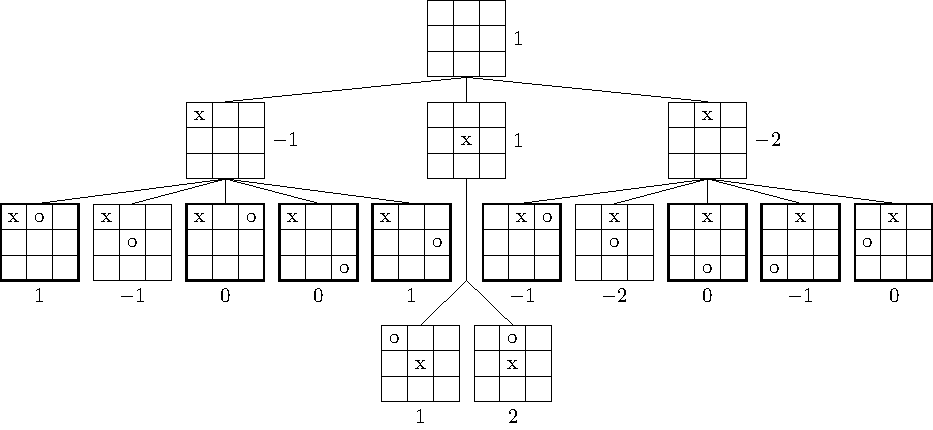
\includegraphics[width=1\textwidth]{forest.pdf}
    \caption{Pohon Permainan dengan Informasi Sempurna}
\end{figure}

\begin{definisi}
    Permainan ekstensif disebut sebagai permainan yang memiliki informasi sempurna apabila tidak ada unsur \textbf{nature}, atau ketika seluruh pemain tahu lokasi \textbf{node} pemain berada ketika bermain.
\end{definisi}

Dalam permainan dinamis, terdapat permainan multitahap yang merupakan jenis permainan lengkap dan tidak sempurna. Permainan multitahap bersifat dinamis karena aksi yang dilakukan kedepannya dapat dipengaruhi oleh aksi yang dilakukan sebelumnya. Permainan \textbf{Persona 4 Golden} adalah contoh permainan multitahap.

%PR 26/04/23
%bahasnya ngikutin slide aja buat flownya
%ceritain tentang contoh yang nyambung ke bentuk teori permainan dengan kelengkapan informasi yg beda" (jadi kasih contoh ada yang infonya lengkap sama gak, dinamis sama gak).
%kalo gak bisa, langsung bikin judulnya aja 
%Teori Permainan berdasarkan Kelengkapan Informasi
%Teori Permainan berdasarkan Bentuk

%mungkin gak kepake
%\begin{definisi}
%    Sebuah fungsi payoff $u : X \rightarrow \mathbb{R}$ merepresentasikan relasi preferensi $\succsim$ jika untuk suatu pasangan $x,y \in X$, $u(x) \geqslant u(y) \Leftrightarrow x \succsim y$
%\end{definisi}






% Bab Studi Literatur digunakan untuk mendeskripsikan kajian literatur yang terkait dengan persoalan tugas akhir. Tujuan studi literatur adalah:

% \begin{enumerate}
%     \item menunjukkan kepada pembaca adanya gap seperti pada rumusan masalah yang memang belum terselesaikan,
%     \item memberikan pemahaman yang secukupnya kepada pembaca tentang teori atau pekerjaan terkait yang terkait langsung dengan penyelesaian persoalan, serta
%     \item menyampaikan informasi apa saja yang sudah ditulis/dilaporkan oleh pihak lain (peneliti/Tugas Akhir/Tesis) tentang hasil penelitian/pekerjaan mereka yang sama atau mirip kaitannya dengan persoalan tugas akhir.
% \end{enumerate}


% \section{Contoh Subbab}
% Perujukan literatur dapat dilakukan dengan menambahkan entri baru di berkas. Tulisan ini merujuk pada \parencite{knuth2001art,vasp1} atau \parencite{4026885} dan \parencite{Kim2006}

% Sekarang mau ke bab berapa yaaaa.... hmm... ke bab \ref{sec:latarbelakang} ahhhhh.

% \blindtext

% \subsection{Contoh Subsubbab}

% \blindtext

% \begin{figure}[h]
%     \centering
%     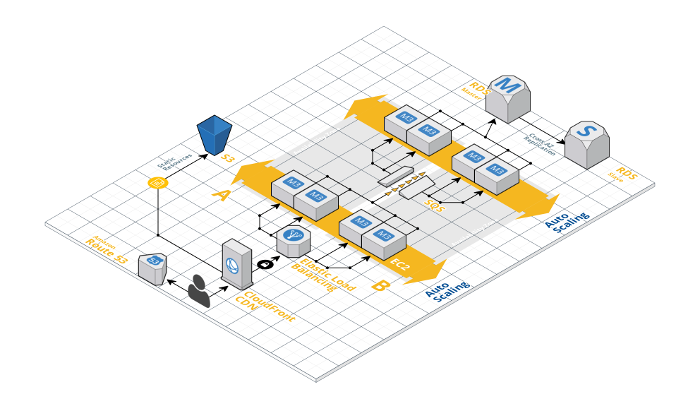
\includegraphics[width=0.8\textwidth]{chapter-2-infrastructure-diagram.png}
%     \caption{Contoh gambar}
% \end{figure}

% \subsubsection{Subsubsubbab}

% \blindtext

% \begin{table}[h]
%     \caption{Tabel random}
%     \vspace{0.25cm}
%     \begin{center}
%         \begin{tabular}{|c|c|c|c|}
%             \hline
%             Title1 & Title2 & Title3 & Title4  \tabularnewline
%             \hline
%             1647   & 1.97   & 0.68   & 1.90 \tabularnewline
%             2301   & 2.92   & 1.06   & 2.75 \tabularnewline
%             2969   & 3.23   & 1.16   & 3.78 \tabularnewline
%             3791   & 4.39   & 1.40   & 4.14 \tabularnewline
%             4625   & 6.72   & 1.87   & 5.59 \tabularnewline
%             \hline
%         \end{tabular}
%     \end{center}
% \end{table}

% \section{Menyisipkan Persamaan}

% Beberapa contoh menyisipkan persamaan.


% \subsection{Contoh Bikin Equation}
% \textbf{text tebal} dan ini \emph{miring}, bikin persamaan di baris yang sama, tinggal pake dolar2 $\Psi(\vec{r}_1,...,\vec{r}_N)$, sehingga persamaan Schr\"{o}dinger, terus, persamaan yang dinomeri kayak gini
% %ini contoh bikin persamaan, ..... :D
% \begin{equation}
%     \left[ \sum_{i}^{N}-\frac{\hbar^2}{2m}\nabla_i^2 + \sum_{i}^{N}V(\vec{r}_i)+ \sum_{i<j}^{N}(\vec{r}_i,\vec{r}_j)\right]\Psi = E\Psi
% \end{equation}

% untuk $N$-elektron, dengan $\hat{H}$=Hamiltonian, $E$=Energi total, $\hat{T}$=Energi kinetik, $\hat{V}$=Energi potensial, dan $\hat{U}$=Interaksi ektron-elektron.

% \subsection{Bikin Matrix}
% Lalalallala.... bikin matrix sekarang, yang ini dikecilin, pake smaller
%     {\smaller
%         \begin{equation}
%             \Psi({\bf r}_1, {\bf r}_2, \cdots {\bf r}_N) = \frac{1}{\sqrt{N!}}\left| \begin{array}{llcl}
%                 \phi_1({\bf r}_1)     & \phi_2({\bf r}_1)     & \cdots                & \phi_N({\bf r}_1)     \\
%                 \phi_1({\bf r}_2)     & \phi_2({\bf r}_2)     & \cdots                & \phi_N({\bf r}_2)     \\
%                 \phi_1({\bf r}_3)     & \phi_2({\bf r}_3)     & \cdots                & \phi_N({\bf r}_3)     \\
%                 \multicolumn{1}{c}{.} & \multicolumn{1}{c}{.} & \multicolumn{1}{c}{.} & \multicolumn{1}{c}{.} \\
%                 \multicolumn{1}{c}{.} & \multicolumn{1}{c}{.} & \multicolumn{1}{c}{.} & \multicolumn{1}{c}{.} \\
%                 \multicolumn{1}{c}{.} & \multicolumn{1}{c}{.} & \multicolumn{1}{c}{.} & \multicolumn{1}{c}{.} \\
%                 \phi_1({\bf r}_N)     & \phi_2({\bf r}_N)     & \cdots                & \phi_N({\bf r}_N)     \\
%             \end{array} \right|
%         \end{equation}
%     }

